\chapter{Wstęp}

Czuwaj!
\begin{floatingfigure}[l]{3cm}
  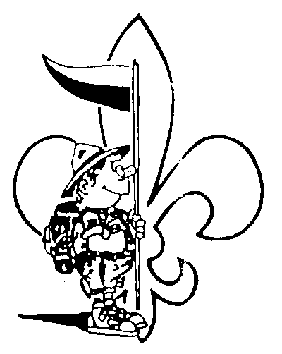
\includegraphics{grafiki/intro.png}
\end{floatingfigure}
Niniejszy skrypt zawiera informacje, które z pewnością przydadzą Ci się w prowadzeniu zastępu. Można go nazwać czymś w rodzaju ściągi. Nie bój się do niego zaglądać, gdy o czymś zapomnisz. Śmiało notuj i podkreślaj te elementy, które są dla Ciebie ważne. Wiedz, że Kurs Zastępowych "Wschód" oraz ten notatnik to tylko wparcie. Najważniejszy jesteś Ty, Twój zapał i chęć działania - to one sprawią, że Twoje zbiórki wyjątkowe a atmosfera w zastępie niepowtarzalna. 

Żeby być dobrym zastępowym, musisz być dobrym harcerzem. Pewnie zadałeś sobie pytanie, po co to całe harcerstwo? Trzeba wiedzieć po co coś robię i dlaczego. To są podstawy. Pamiętaj zatem: celemen naszego pobytu w ZHRze jest wychowywanie metodą harcerską --- w myśl przyrzeczenia i prawa harcerskiego dobrych ludzi. Wszystko inne jest  środkiem do osiągnięcia tego celu. Przypomnijmy sobie fundamenty i podstawy: prawo i przyrzeczenie harcerskie.



\textbf{Przyrzeczenie harcerskie}%wersja ZHR

Mam szczerą wolę całym życiem pełnić służbę Bogu i Polsce, nieść chętną pomoc bliźnim i być posłusznym Prawu Harcerskiemu.


\textbf{Prawo harcerskie}%wersja ZHR
\begin{enumerate}[noitemsep,nolistsep] 
\item Harcerz służy Bogu i Polsce i sumiennie spełnia swoje obowiązki.
\item Na słowie harcerza polegaj jak na Zawiszy.
\item Harcerz jest pożyteczny i niesie pomoc bliźnim.
\item Harcerz w każdym widzi bliźniego, a za brata uważa każdego innego harcerza.
\item Harcerz postępuje po rycersku.
\item Harcerz miłuje przyrodę i stara się ją poznać.
\item Harcerz jest karny i posłuszny rodzicom i wszystkim swoim przełożonym.
\item Harcerz jest zawsze pogodny.
\item Harcerz jest oszczędny i ofiarny.
\item Harcerz jest czysty w myśli, mowie i uczynkach, nie pali tytoniu i nie pije napojów alkoholowych.
\end{enumerate}

